\documentclass{article} % For LaTeX2e

\usepackage{nips14submit_e,times}
\usepackage{hyperref}
\usepackage{url}
\usepackage{graphicx}

\usepackage{listings}
\usepackage{color}

\definecolor{lightgray}{rgb}{1,1,1}
\definecolor{darkgray}{rgb}{.4,.4,.4}
\definecolor{redstrings}{rgb}{0.64,0.08,0.08}
\definecolor{blue}{rgb}{0,0,1}
\definecolor{greencomments}{rgb}{0,0.5,0}
\definecolor{cyan}{rgb}{0.0,0.6,0.6}

\renewcommand{\lstlistingname}{Code fragment}


\lstdefinelanguage{JavaScript}{
  keywords={break, case, catch, continue, debugger, default, delete, do, else, finally, for, function, if, in, instanceof, new, return, switch, this, throw, try, typeof, var, void, while, with, null},
  keywordstyle=\color{blue}\bfseries,
  ndkeywords={class, export, boolean, throw, implements, import, this},
  ndkeywordstyle=\color{blue}\bfseries,
  identifierstyle=\color{black},
  sensitive=false,
  comment=[l]{//},
  morecomment=[s]{/*}{*/},
  commentstyle=\color{greencomments}\ttfamily,
  stringstyle=\color{redstrings}\ttfamily,
  morestring=[b]',
  morestring=[b]"
}

\lstset{
   language=JavaScript,
   backgroundcolor=\color{lightgray},
   extendedchars=true,
   basicstyle=\footnotesize\ttfamily,
   showstringspaces=false,
   showspaces=false,
   numbers=left,
   numberstyle=\footnotesize,
   numbersep=9pt,
   tabsize=2,
   breaklines=true,
   showtabs=false,
   captionpos=b
}


%\documentstyle[nips14submit_09,times,art10]{article} % For LaTeX 2.09


\title{QMiner – Data Analytics Platform for Processing Streams of Structured and Unstructured Data}


\author{
Blaz Fortuna, Jan Rupnik, Carolina Fortuna, Marko Grobelnik, \\
Viktor Jovanoski, Mario Karlovcec, Blaz Kazic, Klemen Kenda, \\
Gregor Leban, Jost Novljan, Miha Papler, Luis Rei, Blaz Sovdat, \\
Luka Stopar, Andrej Muhic \\
Department of Computer Science\\
Jožef Stefan Institute\\
Jamova cesta 39, Ljubljana, Slovenia \\
}

% The \author macro works with any number of authors. There are two commands
% used to separate the names and addresses of multiple authors: \And and \AND.
%
% Using \And between authors leaves it to \LaTeX{} to determine where to break
% the lines. Using \AND forces a linebreak at that point. So, if \LaTeX{}
% puts 3 of 4 authors names on the first line, and the last on the second
% line, try using \AND instead of \And before the third author name.

\newcommand{\fix}{\marginpar{FIX}}
\newcommand{\new}{\marginpar{NEW}}

% \nipsfinalcopy % Uncomment for camera-ready version

\begin{document}


\maketitle

\begin{abstract}
QMiner is an open source analytics platform for performing large scale data analysis written in C++ and exposed via a Javascript API.
The paper presents the main building blocks of the system: storage and index layer, stream aggregates,
feature extractors, linear algebra and analytics, which is followed by a section on the main capabilities and design choices, which
focuses on storage, online processing as well as fast prototyping. Finally, three usage examples are demonstrated with code
fragments: text classification, time series prediction and community detection in graphs.\end{abstract}

\section{Introduction}
QMiner grew out of several EU Framework Programme projects in the areas of text, web, and stream mining over the last couple of years. The developed solutions focus on interactivity and operate on data sets of hundreds of gigabytes in real-time on high-end commodity hardware. These goals and constraints resulted in a unique set of features that we implemented in QMiner.

Applications are implemented in JavaScript, making it easy for novice users to get started. Using the JavaScript API it is easy to compose complete data processing pipelines and integrate with other systems via RESTful web services. The system is based on a C++ library and can be included into custom C++ projects, thus providing them with stream processing and data analytics capabilities.

The system is available as open source project on GitHub under AGPL licence. The repository contains source code, introduction guide and complete documentation of QMiner's JavaScript APIs.

The paper is organised as follows. We first describe the main architectural building blocks, followed by a list of features that, when taken together, uniquely position QMiner in the landscape of open-source analytics packages. We conclude the paper with three examples, which showcase how one can quickly build machine-learning applications.

\section{Building blocks}
The core blocks of the system are:

\textbf{Storage and index layer:} The basic storage abstractions are similar to databases: the data is organized around stores (tables), one data point inside a store corresponds to a record (row or instance) and one record consists of one or more fields (columns or features). Index layer provides support for indexing and retrieving records. Indexes provide support for efficient searching and QMiner provides several types of indexes: (a) inverted index \cite[section 6.5]{knuth1998taocp3}, used to index discrete values and free text, and (b) geo-spatial index, which can be used to index geographic locations presented as longitude and latitude pairs. There are several additional indices in implementation at the moment, which will extend the system: (c) B-tree, used to index linearly ordered data types, such as number and dates, and (d) locality sensitive hashing \cite{har2012approximate}, used to answer nearest neighbour queries on high-dimensional data such as sparse vectors. Indices can be utilized through a JSON-based query languages. The indices are also used by Analytics layer for various tasks, such as describing and extracting features, and for sampling.
\textbf{Stream aggregates:} Aggregates correspond to algorithms which take a stream of records, and maintain some aggregate statistics of the stream. The aggregates connect to a store, and update their state as new records are added to the store. QMiner contains a large collection of stream aggregates, e.g. statistical moments, exponential moving average, resampling and merging of streams, interpolation and extrapolation. In addition, when working in JavaScript API, new stream aggregates can be implemented directly in JavaScript.

\textbf{Feature extractors:} A feature extractor enables mapping records to linear algebra vectors (supports dense and sparse vectors). The core framework for feature extractors enables constructing and gluing several types of feature extractors and automatically performs all the necessary bookkeeping. Feature extractors include: numeric feature extractors, text feature extractors (bag of words), element indicator vectors and set indicator vectors (multi-label). In addition, when working with the JavaScript API, custom feature extractors can be implemented as JavaScript functions.

\textbf{Linear algebra:} The library includes manipulation of several implementations of vectors and matrices. Algorithms enable solving linear systems and computing several matrix decompositions. Randomized algorithms enable solving large scale problems, such as singular value decompositions\cite{tropp} on large structured or sparse matrices. The QMiner library can optionally
be compiled with optimized Basic Linear Algebra libraries such as Intel MKL.
\textbf{Analytics:} The analytics components combine all above components to implement various popular machine learning algorithms for clustering, dimensionality reduction, classification, regression and active-learning. The implementations can be easily applied directly to data stored in the storage layer. The analytics components can either be implemented purely in C++ or alternatively in JavaScript, by using core C++ modules (such as linear algebra) to retain efficiency.


\section{Features}
In this section we provide an overview of the main features of QMiner.

\textbf{Connecting storage, indexing and analytics:} QMiner stores and indexes the data in a way that makes the implemented machine learning methods more scalable. Computing feature vectors from stored records aims at reducing duplication of data in the process and relies heavily on the integrated indexing and its features (e.g. probabilistic joins) to speed up transformations. Data schemas provide types for directly storing vectors and sparse vectors as part of records.

\textbf{Multi-modal data support:} QMiner provides native support for handling and learning from unstructured data such as text or graphs. Among the supported data operations are full text search, aggregation over text fields, creation and storage if bag-of-words vectors directly in the data stores, and full integration of Stanford graph analysis library SNAP \cite{snap} in the C++ and JavaScript APIs. Additionally several time series tools (resampling, merging, computing moments, extrapolation, interpolation, discretization) are implemented.

\textbf{Streaming processing:} QMiner provides building blocks for processing and learning from streams of text documents, website logs or numeric streams. For example, pipeline-able stream aggregates for maintaining aggregate statistics over the stream, and machine learning algorithms for learning from stream.

\textbf{Probabilistic joins between tables:} For some operations computing a complete join between tables is not necessary. For example, to compute the gender distribution of visitors of a particular web page, we do not really need a complete list of visitors for that particular web page. What suffices is a statistically representative sample. QMiner supports several sampling techniques for achieving this, and integrates the support for probabilistic joins in query language and feature extractors.

\textbf{Efficiency and fast prototyping:} All main components of the library are implemented in C++ and are optimized for memory usage and computational speed. This involves the data store, indexing, feature extractors, linear algebra, stream processing components, several machine learning and graph mining algorithms (based on SNAP library). Most of the core functionality is exposed in the JavaScript API which enables fast prototyping and deploying as RESTful services, since
QMiner can operate as an HTTP server.


\section{Examples}

QMiner lets you get from data to working models exposed through web service API in less than an hour. Most applications can be scripted fully in the JavaScript layer, taking advantage of components implemented in C++ and libraries such as Intel MKL. We will demonstrate the system on three different tasks: text classification, time series prediction and community detection on graphs.

\subsection{Text processing, classification and regression}

The example in this section demonstrates how to extract features from the movie dataset to build classification models to predict movie genre.

First, we import the analytics module which provides machine learning algorithms. Next, we load the data and enumerate features we would like to extract from the data set. For each feature we need to specify its type (for example, \texttt{text}), its source (for example, \texttt{Movies}), and name (for example, \texttt{plot}). (Source is the \emph{data store} from which we want to extract the feature) We can now run batch learner that returns the model that tries to predict movie genres using the whole data set for training (in this case, the model is stored in the \texttt{genreModel} variable). Once we saved the model we can easily use it for prediction (for example, \texttt{var newGenre = genreModel.predict(newMovie);}).

      \begin{lstlisting}[caption={Text mining: storage, feature extraction and classification.}] 	
      // Import analytics module
      var analytics = require("analytics.js");
      // Loading in the dataset.
      qm.load.jsonFile(Movies, "./sandbox/movies/movies.json");
       	
      // Declare the features we will use to build genre classification models
      var genreFeatures = [
          { type: "constant", source: "Movies" },
          { type: "text", source: "Movies", field: "Title" },
          { type: "text", source: "Movies", field: "Plot" },
          { type: "join", source: { store: "Movies", join: "Director"} }
      ];
      // Create a model for the Genres field, using all the movies as training set.
      var genreModel = analytics.newBatchModel(
         Movies.recs, genreFeatures, Movies.field("Genres"));
      // Predict genres of a new movie
      var newMovie = qm.store("Movies").newRec({
         Title:"Unnatural Selection",
         Plot:"When corpses are found with organs missing ...",
         Genres:["Horror", "Sci-Fi"],
         Director:{Name:"Baggs Bill", Gender:"Unknown"}
      });
      var predictedGenre = genreModel.predict(newMovie);
      \end{lstlisting}

\subsection{Time series processing}

The following example demonstrates how to perform time series prediction. The example uses stream aggregates (rounded rectangles in Figure \ref{fig:timeSeries}) to first resample incoming time series into a equaly spaced time series, on which two exponential moving averages (EMAs) are computed. To learn the prediction model we construct a feature vector containing the numeric value, the two EMAs and the date features (time of day, day of week, month) and send it to incremental linear regression model. A 1 minute delay operator is applied to the input
 variables, which corresponds to a 1 minute prediction horizon.

The example involves two \emph{data stores}: \texttt{Raw} and \texttt{Resampled}. The records from the \texttt{Raw} data store represent time series measurement pairs (timestamp, value) and \texttt{Resampled} stores the resampled time series, together with the results of two smoothers. Each time a record is added to \texttt{Raw} we update the resampler. The resampler may insert a record in
\texttt{Resampled} based on the interpolation used. Each time a record is added to \texttt{Resampled} several operations are executed: computation of two smoothers, update of the delay operator, enrichment of the resampled record with the results of the smoothers, and the update of the linear regression model.

      \begin{figure}[h]
      \begin{center}
      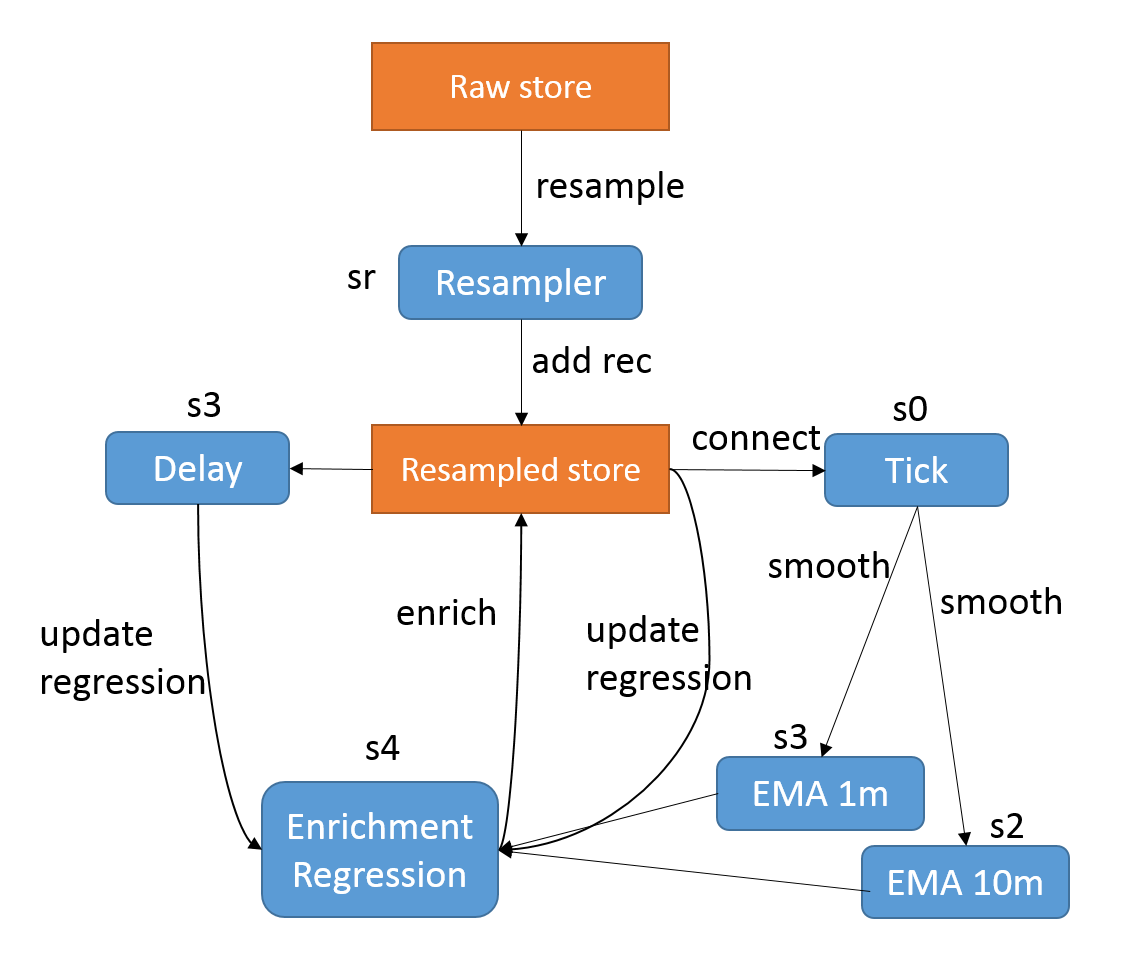
\includegraphics[width=0.5\textwidth]{timeSeries2.PNG}
      \end{center}
      \caption{Time series processing architecture}\label{fig:timeSeries}
      \end{figure}

      \begin{lstlisting}[caption=Time series processing] 	


      // Here we connect several stream aggregates to the stores: a resampler, a connector, two smoothers with different decays and a delay operator. These correspond to blue boxes in figure 1.
      var sr = Raw.addStreamAggr({name: "Resamp10s", type: "resampler",
          outStore: "Resampled"/*, resampling params*/});
      var s0 = Resampled.addStreamAggr({name: "tick", type: "timeSeriesTick"/*, aggregate params*/});
      var s1 = Resampled.addStreamAggr({name: "EMA1m", type: "ema", interval: 60000/*, aggregate params*/});
      var s2 = Resampled.addStreamAggr({name: "EMA10m", type: "ema", interval: 600000/*, aggregate params*/});
      var s3 = Resampled.addStreamAggr({ name: "delay", type: "recordBuffer", size: 6 });

      // Declare features from the resampled timeseries
      var ftrSpace = analytics.newFeatureSpace([
          { type: "numeric", source: "Resampled", field: "Value" },
          { type: "numeric", source: "Resampled", field: "Ema1" },
          { type: "numeric", source: "Resampled", field: "Ema2" },
          { type: "multinomial", source: "Resampled", field: "Time", datetime: true }
      ]);
      // Initialize linear regression model
      var linreg = analytics.newRecLinReg(/*params */);

      // We add the final stream aggregate that enriches the record and updates the regression model
      var s4 = Resampled.addStreamAggr(new function(){
          onAdd: function (rec) {
              // Enrich record
              rec.Ema1 = s1.getFlt();
              rec.Ema2 = s2.getFlt();
              // Get the id of the record from a minute ago.
              var trainRecId = s3.val.last;
              // Update the regression model: the input is delayed by 1 minute and the output is the current value
              linreg.learn(ftrSpace.ftrVec(Resampled[trainRecId]), rec.Value);
          }
      });
      \end{lstlisting}


\subsection{Graph analysis}
QMiner supports handling of graph data by providing JavaScript API for the integrated SNAP library \cite{snap}.
The script in Code fragment 3 is an example of loading a graph, computing communities and visualizing the results.

After importing the required modules for graph analysis and visualization, an edge-list graph file is loaded into a new undirected graph. The graph represents co-authoring network of Slovenian researchers from biotechnical science in 2013. Nodes of the graph represent researchers, while edges between nodes indicate co-authoring of at least on publication. Real networks often have community structure with several regions of internally densely connected nodes. Communities in co-authoring network can indicate groups of strongly connected researchers from a research lab or a similar organization, or simply groups of scientist with a common research interest. Number, sizes and connectivity between communities reveals the cohesiveness of a network. Following the simplification of the graph by removing weekly connected nodes (with degree 3 or less), the Clauset-Newman-Moore \cite{clauset-newman-moore} community detection algorithm is applied to compute communities. In the final step the graph is plotted using force-directed layout, with node colors corresponding to communities. The complete script in Code fragment 3 is written in JavaScript, but some of the components, such as community detection algorithm are executing in highly optimized C++ SNAP code.
\begin{figure}[h]
\begin{center}
\includegraphics[scale=0.20]{communities_labeled.jpg}
\caption{Communities of co-authoring graph}
\end{center}
\end{figure}
      \begin{lstlisting}[caption=Graph analysis]
      // Import snap module.
      snap = require("snap.js");
      // Import visualization module.
      viz = require("visualization.js");
      // Loading a graph file and creating a new undirected graph.
      var g = snap.newUGraph("biotechnology_2013.edg");
      // Simplifying graph by removing all the nodes with degree
      // smaller or equal to 3.
      var g = snap.removeNodes(g, 3);
      // computing communities using Clauset-Newman-Moore algorithm
      var CmtyCNM = snap.communityDetection(g, "cnm");
      // plotting the graph with colors of colors corresponding to communities
      viz.drawGraph(g, "graphCNM.html", { "color": CmtyCNM });
      \end{lstlisting}
The results of analysis shows that the co-authoring graph has 12 communities labeled from 1 to 12 in Figure 2. Three smaller communities (10, 11 and 12) are completely disconnected, while the rest make a connected component. By supporting SNAP, QMiner enables further rich graph analysis in a easy to use JavaScript interface, which can be especially useful when combined with the supported scalable machine learning methods.

\subsection{Conclusion}
This paper presents QMiner, an open source analytics platform for performing large scale data analysis. The system is build from five architectural modules and has several desirable features, including: connecting storage, indexing and analytics, scalability of implemented machine learning methods, multimodal data support, processing of streaming data, probabilistic joins between tables and fast as well as scalable prototyping.

Architecture of the system with core implemented in C++ and JavaScript layer on top of it enables ease of use, without sacrificing performance. As illustrated with examples of text classification, time series processing and graph analysis, complete workflows can be implemented with simple scripts.

\subsubsection*{Acknowledgments}
The research leading to these results has received funding from the European Union Seventh Framework Programme (FP7/2007-2013) under grant agreement no 317534 (the Sophocles project) as well as the project X-LIKE (ICT-257790-STREP)\cite{xlike} and SYMPHONY FP7 Collaborative project (FP7-ICT-611875).


\bibliographystyle{unsrt}
\bibliography{qminer}

\end{document}